% !TEX root = ../report_template.tex
\section{Baseline and evaluation}\label{sec:evaluation}
% 3 points.

\subsection{Baseline models}\label{sec:baselines}
% Simple baselines fitted per table (k-NN, linear models, random forests,
% gradient-boosted trees) and the first approach from our prototype.
% Why these? Introduce the prototype briefly here; the paper's method is
% explained in \Cref{sec:method}.

\todo{baselines and the prototype, and why}

\subsection{Evaluation metrics and protocol}\label{sec:metrics}
% Which metrics are meaningful, and why?
% Protocol: splits, rows per dataset, which datasets are skipped.
% How do we aggregate over many datasets of different difficulty?

\todo{metrics, protocol and aggregation}

\subsection{Experimental results}\label{sec:results}
% Training and validation loss curves of the prototype; baselines vs.
% prototype on synthetic and real tables, broken down by relevant
% categories (e.g. number of classes, rows, features).
% Captions only describe; the interpretation goes in the text.

\begin{figure}
  \centering
  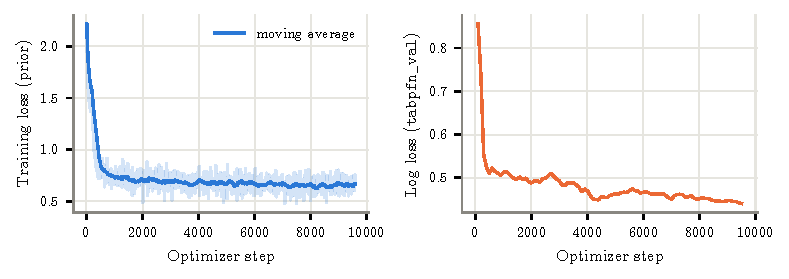
\includegraphics[width=\linewidth]{training_curves}
  \caption{Training loss on the prior (left) and log loss on the \tabpfnval{}
    datasets (right) over the optimizer steps of the 2-hour run.}
  \label{fig:training_curves}
\end{figure}

\Cref{fig:training_curves} shows \todo{what can be seen, and does it make sense?}

% Table pattern (booktabs, best value in bold):
% \begin{table}
%   \centering
%   \begin{tabular}{lrrr}
%     \toprule
%     Method & Log loss & Accuracy & ROC AUC \\
%     \midrule
%     Prototype (ours) & \textbf{0.44} & 0.84 & 0.89 \\
%     Random forest    & 0.50 & 0.82 & 0.87 \\
%     \bottomrule
%   \end{tabular}
%   \caption{Mean scores on the \tabpfnval{} datasets. Best value in bold.}
%   \label{tab:baselines}
% \end{table}

\subsection{Overfitting and failure analysis}\label{sec:overfitting}
% Is overfitting an issue? How do we check for it, and how do we avoid it?
% Where do the baselines and the prototype fail?

\todo{overfitting; where the methods fail}

\subsection{Non-technical view}\label{sec:nontechnical}
% What makes the task easy or hard, in plain words?

\todo{what makes the task easy or hard}
